\problemname{Flight Plan Evaluation}

%\illustration{0.42}{sample1}{The second sample input}
When flying between two places, constructing a good flight plan is
important.  In general there is a wide range of different factors to
consider, the most important being fuel consumption and weather
forecasts (especially winds).  In this problem, we will evaluate
flight plans with respect to a third statistic, namely how much of the
flight is over water, and how much is over ground.  This statistic is
not relevant per se, yet many passengers seem to prefer flying over
land -- either because they are afraid of flying over water, or simply
because the view tends to be slightly more interesting when flying
over land.

For this problem, we assume that the earth is a perfect sphere with
radius $6370$ km.  We model each continent of the earth as a polygon
on this sphere -- a closed sequence of line segments, where a line
segment between two points consists of the shortest spherical arc
between these two points.  The two end-points of a line segment can
not be the same point, or antipodal (diametrically opposite) points.
Similarly a flight route is modeled as a sequence of waypoints
connected by line segments, but unlike the line segments of a polygon
these line segments may cross themselves and will not necessarily end
up where they started.

\begin{figure}[!h]
  \centering
  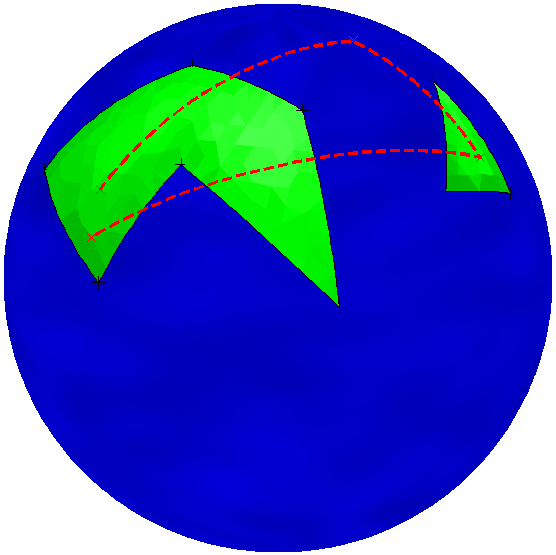
\includegraphics[width=0.55\textwidth]{sample1}
  \caption{The second sample input}
\end{figure}

In order to simplify the problem, we additionally make the following
two assumptions:
\begin{itemize}
\item No waypoint of a flight route lies within $0.1$ km of any shoreline (a line segment that is part of a polygon).
\item No vertex of any continent polygon lies within $0.1$ km of the flight route.
\end{itemize} 

All coordinates on the sphere are represented as a pair of latitude and
longitude (both in degrees).  A point with latitude $\pm 90$ is the
north/south pole, and points with latitude $0$ are the points on the
equator.

\section*{Input}

The input consists of:

\begin{itemize}
\item one line with an integer $1 \le c \le 30$, the number of continents;
\item $c$ lines, each describing a continent. Each such line starts
  with an integer $3 \le n \le 30$, the number of vertices in the
  polygon describing the continent.  This is followed by $n$ pairs of
  integers $\phi_1, \lambda_1, \ldots, \phi_n, \lambda_n$, where $-90
  \le \phi_i \le 90$ and $0 \le \lambda_i \le 359$ are the latitude and
  longitude of the $i$th vertex of the continent;
\item one line describing the flight plan.  The line starts with an
  integer $2 \le m \le 30$, the number of waypoints.  This is followed
  by $m$ pairs of integers $\phi_1, \lambda_1, \ldots, \phi_m,
  \lambda_m$, where $-90 \le \phi_i \le 90$ and $0 \le \lambda_i \le
  359$ are the latitude and longitude of the $i$th waypoint of the
  route.
\end{itemize}

A continent cannot cross itself.  No continent will touch or contain
any other continent.  Continents are given in counterclockwise order,
in the sense that
if you go from the first vertex of the polygon to
the second one, the interior of the continent is on your left hand
side.
%if the first point of a continent is $P$, and the
%second one is $Q$, then the interior of the continent is on the left
%side when going from $P$ to $Q$.

The first and last waypoints of the route will always be inside a
continent (but not necessarily the same continent).

\section*{Output}

Output two real numbers $l$ and $w$, where $l$ is
the total length of the flight (in km), and $w$ is the percentage of
the flight that is over water.  The numbers should be accurate to an
absolute or relative error of at most $10^{-6}$.
